\documentclass[10pt,utf8]{beamer}

\mode<presentation> {
%  \usetheme{Boadilla}
  \usetheme{Madrid}
%	\usetheme{Fzu}
  \setbeamercovered{transparent}
}

\usepackage{palatino}
\usepackage{graphicx}
\usepackage{array}
\usepackage{color}
\usepackage{subfigure}
\usepackage{colortbl}
\usepackage{amsmath}
\usepackage{hyperref}
\usepackage{listings}
\usepackage{fancyvrb}

\setbeamertemplate{caption}{\raggedright\insertcaption\par} %turn off caption prefix ("Figure")

\title{Ideas behind sanlock}
\author{Vojtěch Juránek}
\institute[Red Hat]{Red Hat}
\date{25.~1.~2020, DevConf.CZ, Brno}

\lstdefinestyle{Bash}{
	basicstyle          = \large\ttfamily,
	language            = Bash,
	numbers             = left,
	numberstyle         = \small,
	stepnumber          = 1,
	numbersep           = 5pt,
	backgroundcolor     = \color{white},
	showspaces          = false,
	showstringspaces    = false,
	showtabs            = false,
	frame               = single,
	tabsize             = 2,
	captionpos          = b,
	breaklines          = true,
	breakatwhitespace   = false,
	morestring          = [b]",
	stringstyle         = \color{blue},
	keywordstyle        = \color{magenta},
	commentstyle        = \color{gray},
	identifierstyle     = \color{black},
	moredelim           = **[is][\bfseries]{`}{`},
	moredelim           = **[is][\color{magenta}]{!}{!}, 
	fancyvrb            = true,
}


\begin{document}

\begin{frame}
    \titlepage
\end{frame}

\begin{frame}
    \frametitle{Storage area network}
    \begin{figure}
        \centering
        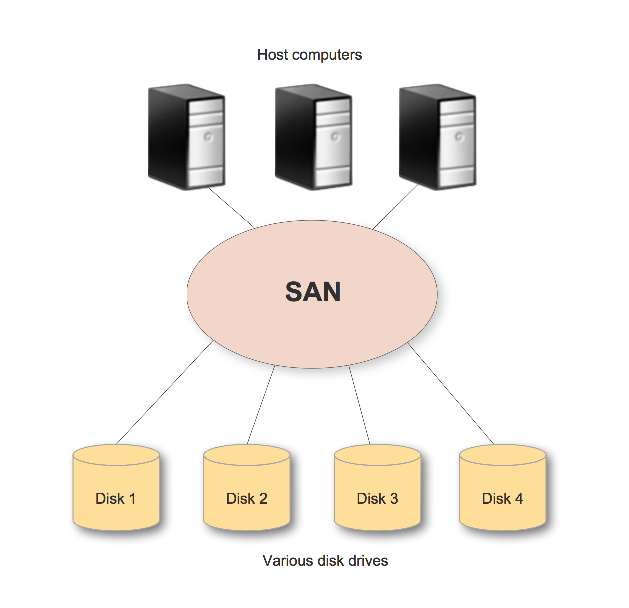
\includegraphics[height=7cm]{./img/san.eps}
        \caption{\tiny{Source: \url{https://www.ibm.com/developerworks/community/wikis/
        %\caption{\tiny{Source: \url{https://www.ibm.com/developerworks/community/wikis/home?lang=en\#!/wiki/IBM\%20Technology\%20Made\%20Simple/page/Storage\%20Virtualization\%20Technology
        }}}
    \end{figure}
\end{frame}

\begin{frame}
    \frametitle{Storage virtualization}
    \begin{figure}
        \centering
        
\includegraphics[height=5cm]{./img/virt-storage.eps}
        \caption{\tiny{Source: \url{https://sharedstorage.wordpress.com/2017/01/03/storage-virtualization/}}}
    \end{figure}
\end{frame}

\begin{frame}
 \frametitle{Data consistency}
 \begin{figure}
    \centering
    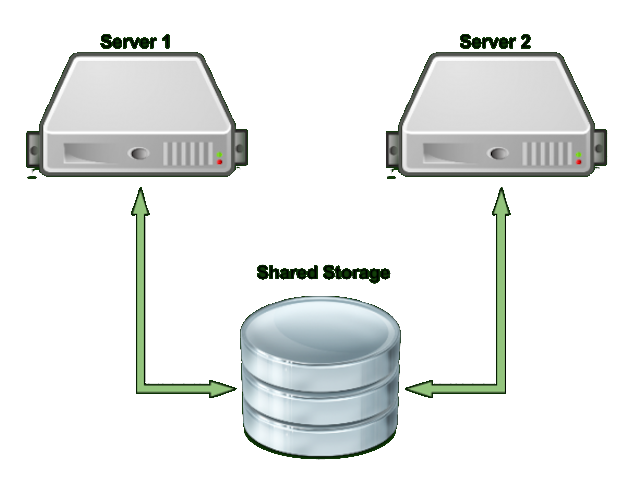
\includegraphics[height=5cm]{./img/disk-paxos.eps}
    \caption{\tiny{Source: \url{https://www.linuxjournal.com/content/high-availability-storage-ha-lvm}}}
 \end{figure}
\end{frame}

\begin{frame}
 \frametitle{Data consistency}
 \centering
 \Large{Dedicated (external) lock manager:}
 \begin{figure}
    \centering
    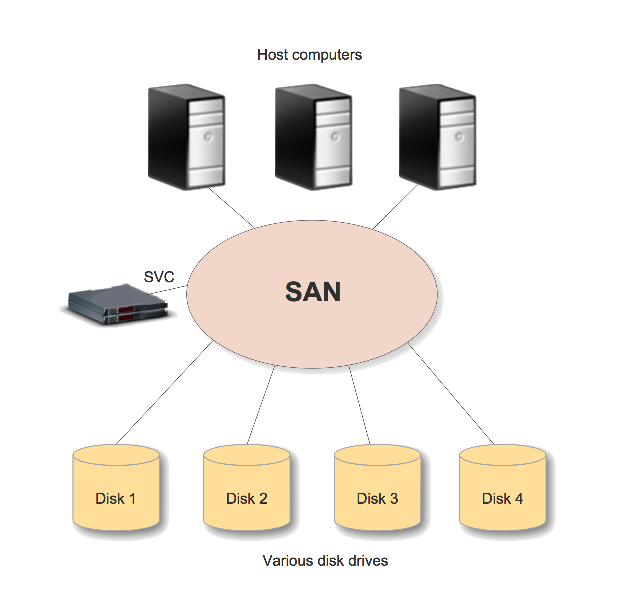
\includegraphics[height=6cm]{./img/san-svc.eps}
    \caption{\tiny{Source: \url{https://www.ibm.com/developerworks/community/wikis/
    %\caption{\tiny{Source: \url{https://www.ibm.com/developerworks/community/wikis/home?lang=en\#!/wiki/IBM\%20Technology\%20Made\%20Simple/page/Storage\%20Virtualization\%20Technology
    }}}
 \end{figure}
\end{frame}

\begin{frame}
 \frametitle{Data consistency}
 \centering
 \Large{What about co-locate locks with the data and access the locks together with accessing the data itself.}
\end{frame}


\begin{frame}
    \frametitle{sanlock}
    \begin{itemize}
     \item \color{blue}\url{https://pagure.io/sanlock}\color{black}
     \item Shared storage lock manager.
     \item Build on top of Disk Paxos and $\Delta$-Leases algorithms.
    \end{itemize}
\end{frame}

\begin{frame}
    \frametitle{Refresh: Basic Paxos}
    \begin{figure}
        \centering
        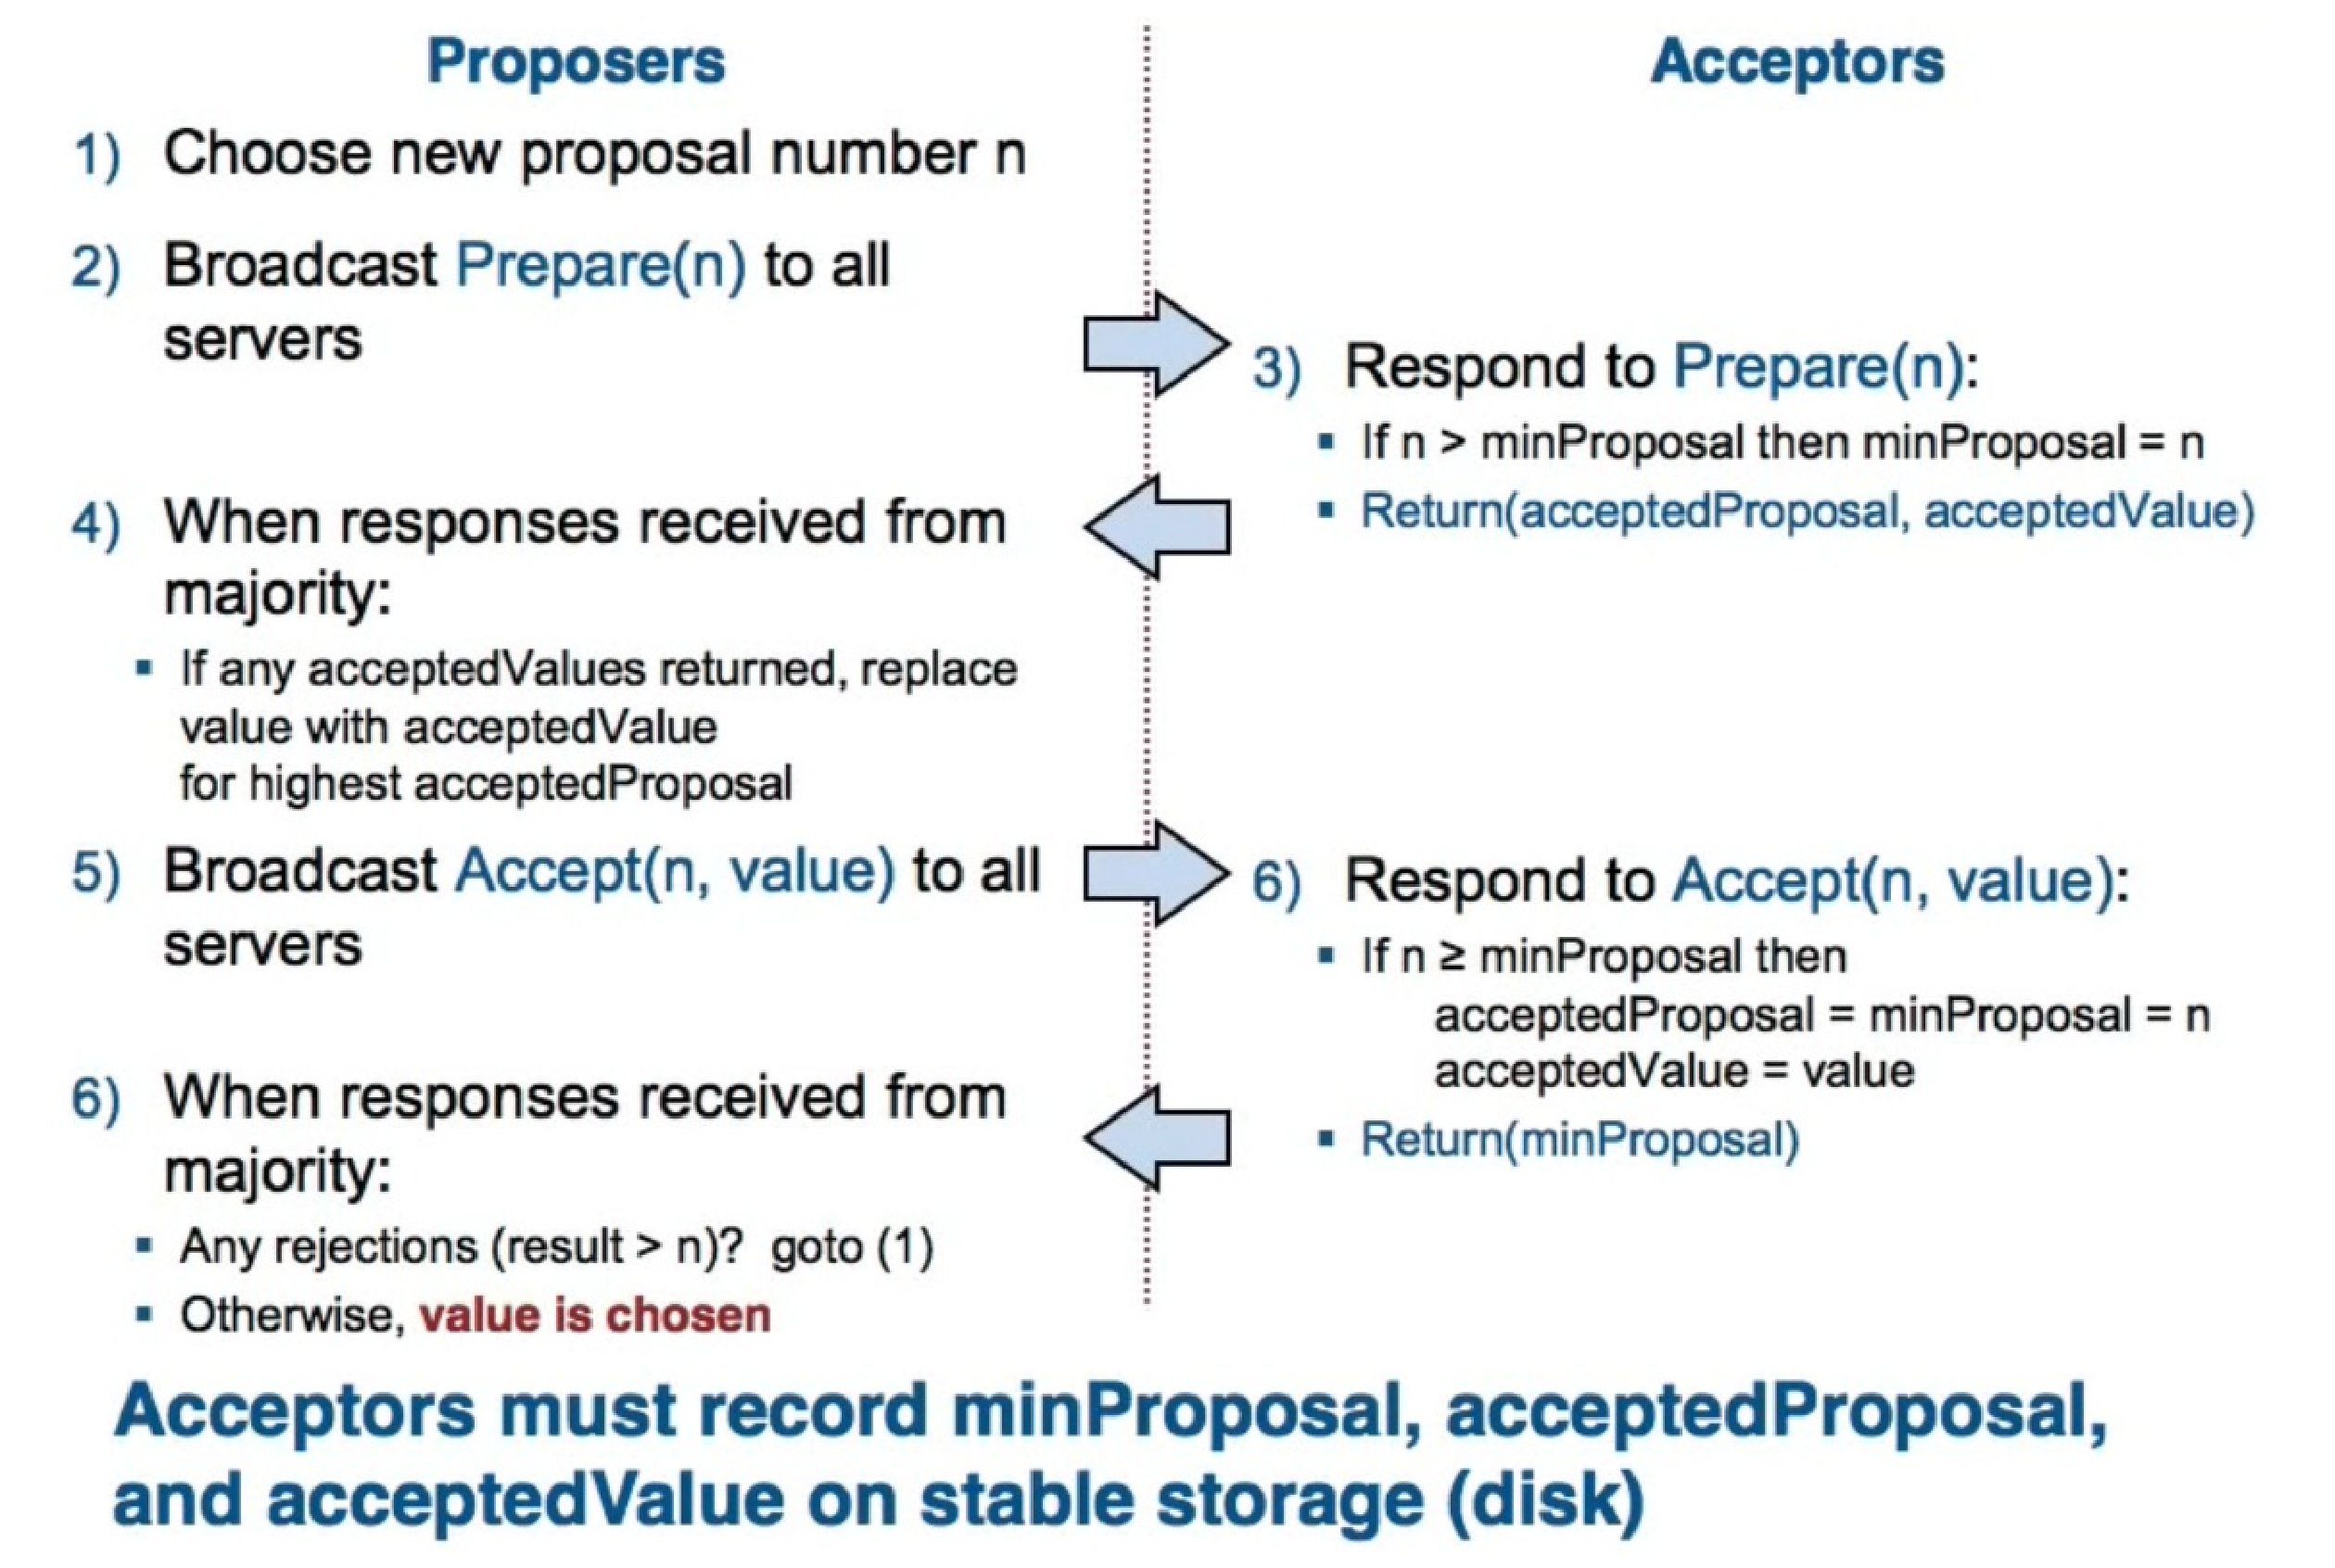
\includegraphics[height=7cm]{./img/basic-paxos.eps}
        \caption{\tiny{Source: \url{https://youtu.be/JEpsBg0AO6o?t=1050}}}
    \end{figure}
\end{frame}

\begin{frame}
    \frametitle{Disk Paxos}
    \begin{figure}
        \centering
        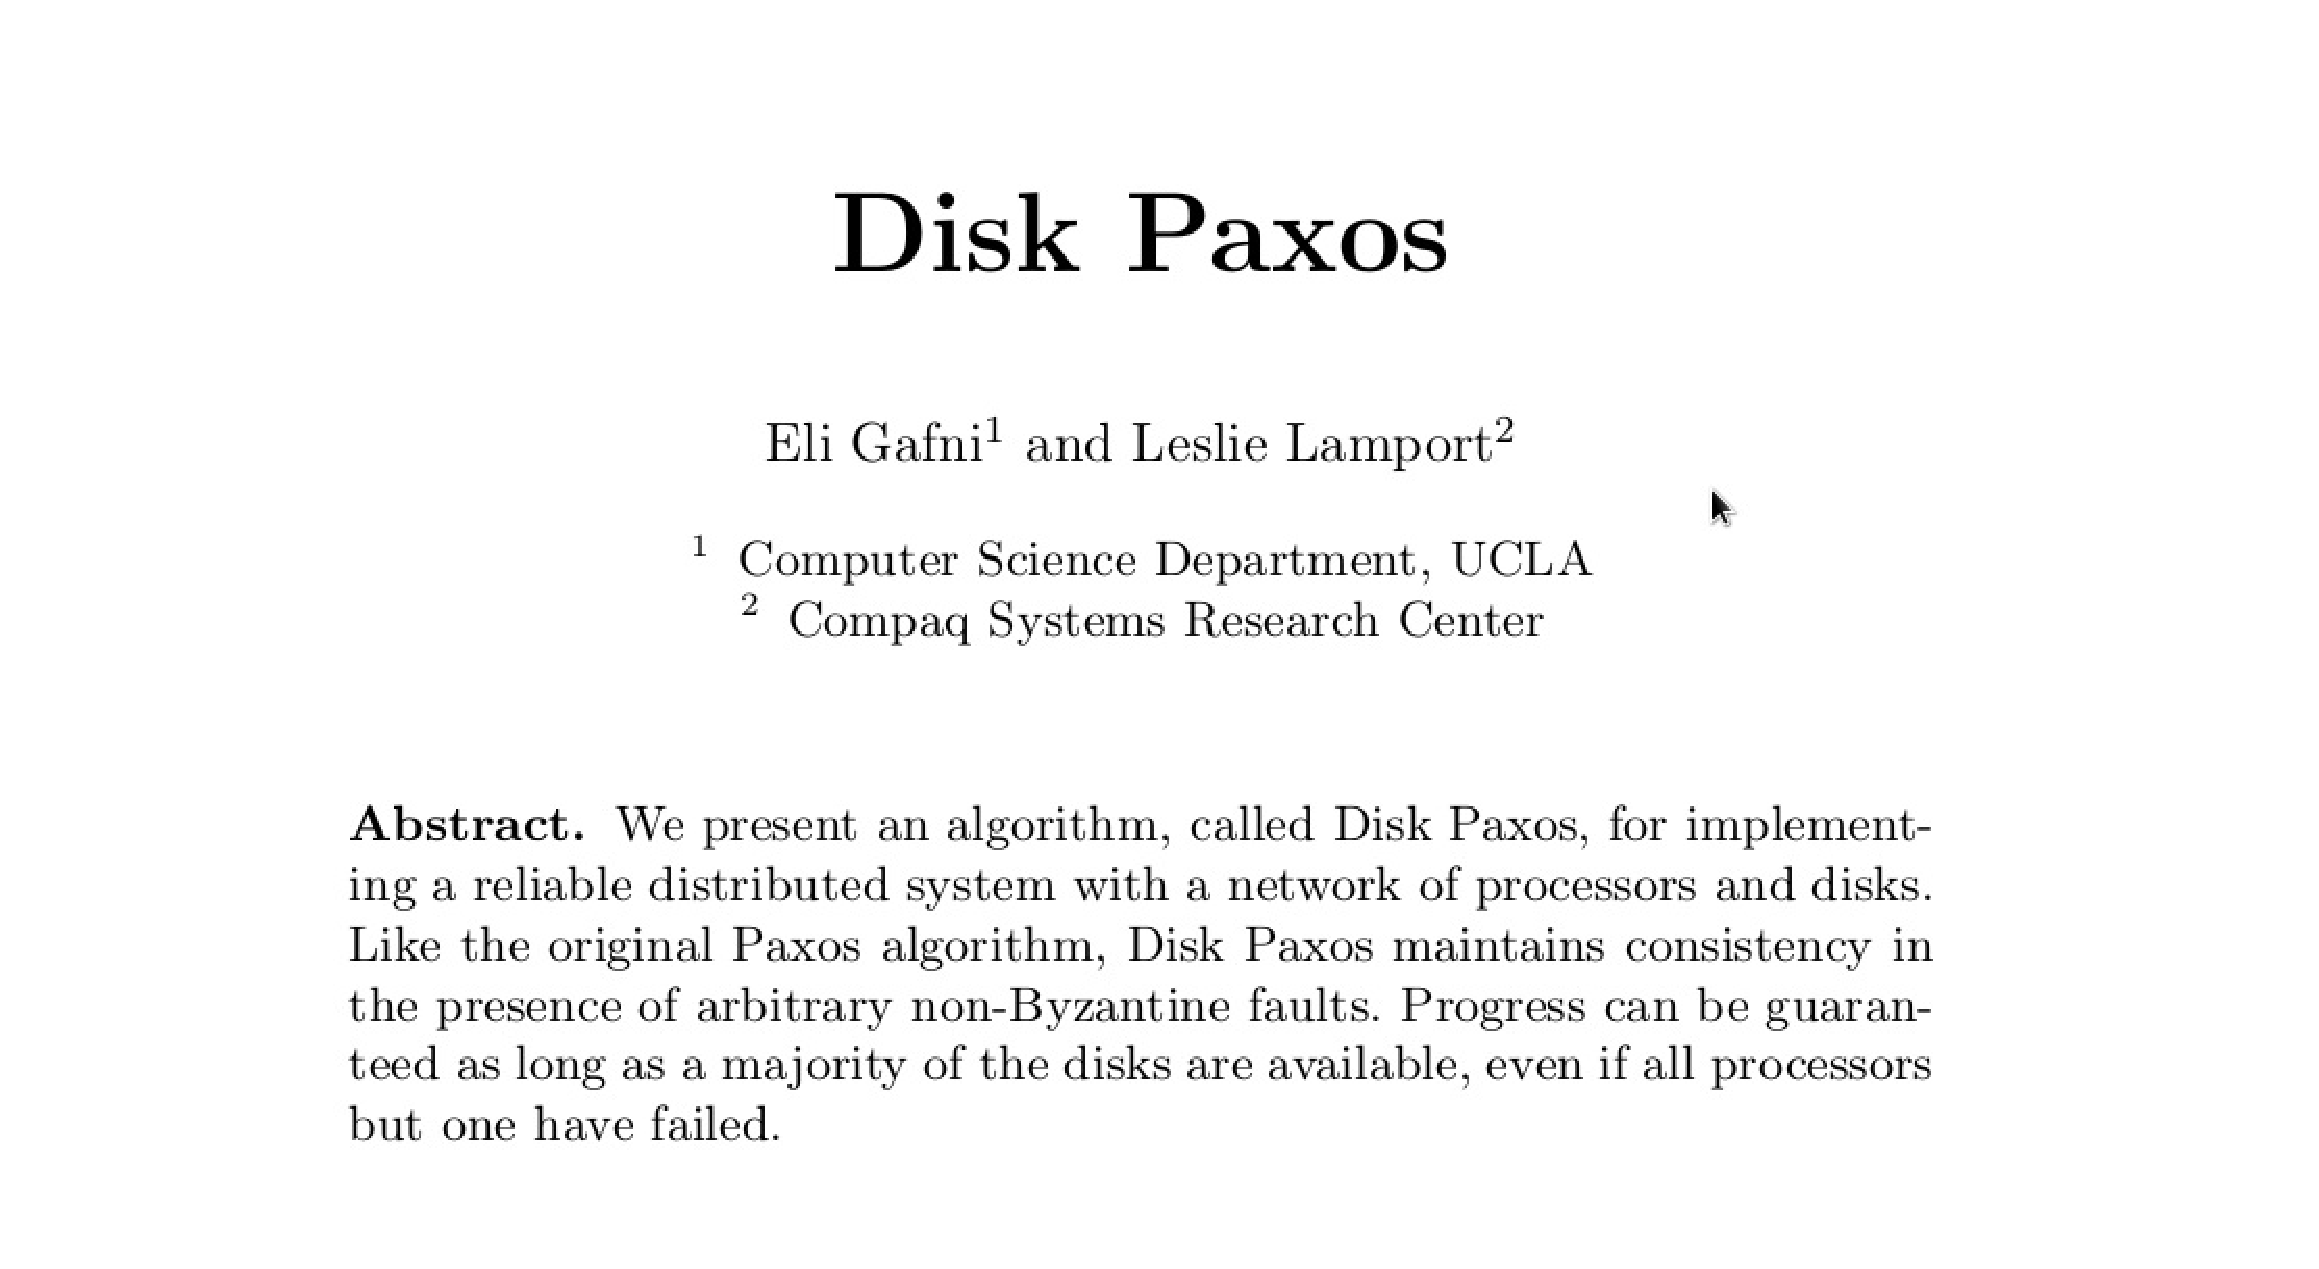
\includegraphics[height=5cm]{./img/disk-paxos-paper.eps}
    \end{figure}
\end{frame}

\begin{frame}
    \frametitle{Disk Paxos}
    \centering
    \textbf{In whole algorithm we assume reading and writing are atomic operations.}\\
    \vspace{1cm}
    
    \begin{itemize}
     \item Assume we have \texttt{m} disks \texttt{d} and \texttt{n} processors (computers) \texttt{p}.
     \item Each processor has an assigned block on each disk.
     \item Each processor stores on assigned block on each disk following structure \texttt{dblock[p]}:
     \begin{itemize}
        \item \texttt{mbal} - ballot number
        \item \texttt{bal} - largest ballot number for which \texttt{p} reached preparing commit phase
        \item \texttt{inp} - value \texttt{p} tries to commit in ballot \texttt{bal}
     \end{itemize}
    \end{itemize}
\end{frame}


\begin{frame}
    \frametitle{Phase 1: proposing a value}
    \centering
    \textbf{For each disk \texttt{d}}
    \vspace{0.5cm}
    \begin{itemize}
        \item write \texttt{dblock[p]} to disk \texttt{[d][p]}
        \item read \texttt{dblock[p]} from \texttt{[d][q]} for all other processes \texttt{[q]}
    \end{itemize}
    
    \vspace{1cm}
    
    \centering
    \textbf{For any disk \texttt{d} and process \texttt{q}:}
    \vspace{0.5cm}
    \begin{itemize}
        \item if \texttt{[d][q].mbal > dblock[p].mbal} $\rightarrow$ abort
        \item else if read majority of disks $\rightarrow$ phase finished
    \end{itemize}
\end{frame}

\begin{frame}
    \frametitle{Phase 2: preparing the commit of a value}
    \centering
    \textbf{Choosing a value:}
    \vspace{0.5cm}
    \begin{itemize}
     \item \texttt{inp = dblock[q].inp}, where \texttt{dblock[q]} is block with largest \texttt{dblock[q].bal} among read blocks
     \item or value proposed by \texttt{p} is all read blocks haven't any value set
    \end{itemize}
\end{frame}

\begin{frame}
    \frametitle{Phase 2: preparing the commit of a value}
    
    \centering
    \textbf{For each disk \texttt{d}}
    \vspace{0.5cm}
    \begin{itemize}
        \item write \texttt{dblock[p]} to disk \texttt{[d][p]}
        \item read \texttt{dblock[p]} from \texttt{[d][q]} for all other processes \texttt{[q]}
    \end{itemize}
    
    \vspace{1cm}
    
    \centering
    \textbf{For any disk \texttt{d} and process \texttt{q}:}
    \vspace{0.5cm}
    \begin{itemize}
        \item if \texttt{[d][q].mbal > dblock[p].mbal} $\rightarrow$ abort and start phase 1 with higher ballot number
        \item else if read majority of disks $\rightarrow$ value committed, broadcast it
    \end{itemize}
\end{frame}

\begin{frame}
    \frametitle{Broadcasting a value}
    \centering
    If \texttt{p} learns that some other value was committed during the process $\rightarrow$ abort and output committed value.
\end{frame}


\begin{frame}
 \frametitle{Unsolved problems}
 \begin{itemize}
  \item How to add processors.
  \item How to store location/mapping of processors on the disks.
 \end{itemize}
\end{frame}

\begin{frame}
 \frametitle{Other problems}
 \centering
 \begin{figure}
        \centering
        
\includegraphics[height=7cm]{./img/howard_disk_paxos.eps}
        \caption{\tiny{Source: \url{https://twitter.com/heidiann360/status/1189137985830297600}}}
    \end{figure}
\end{frame}


\begin{frame}
    \frametitle{$\Delta$-Lease}
    \begin{figure}
        \centering
        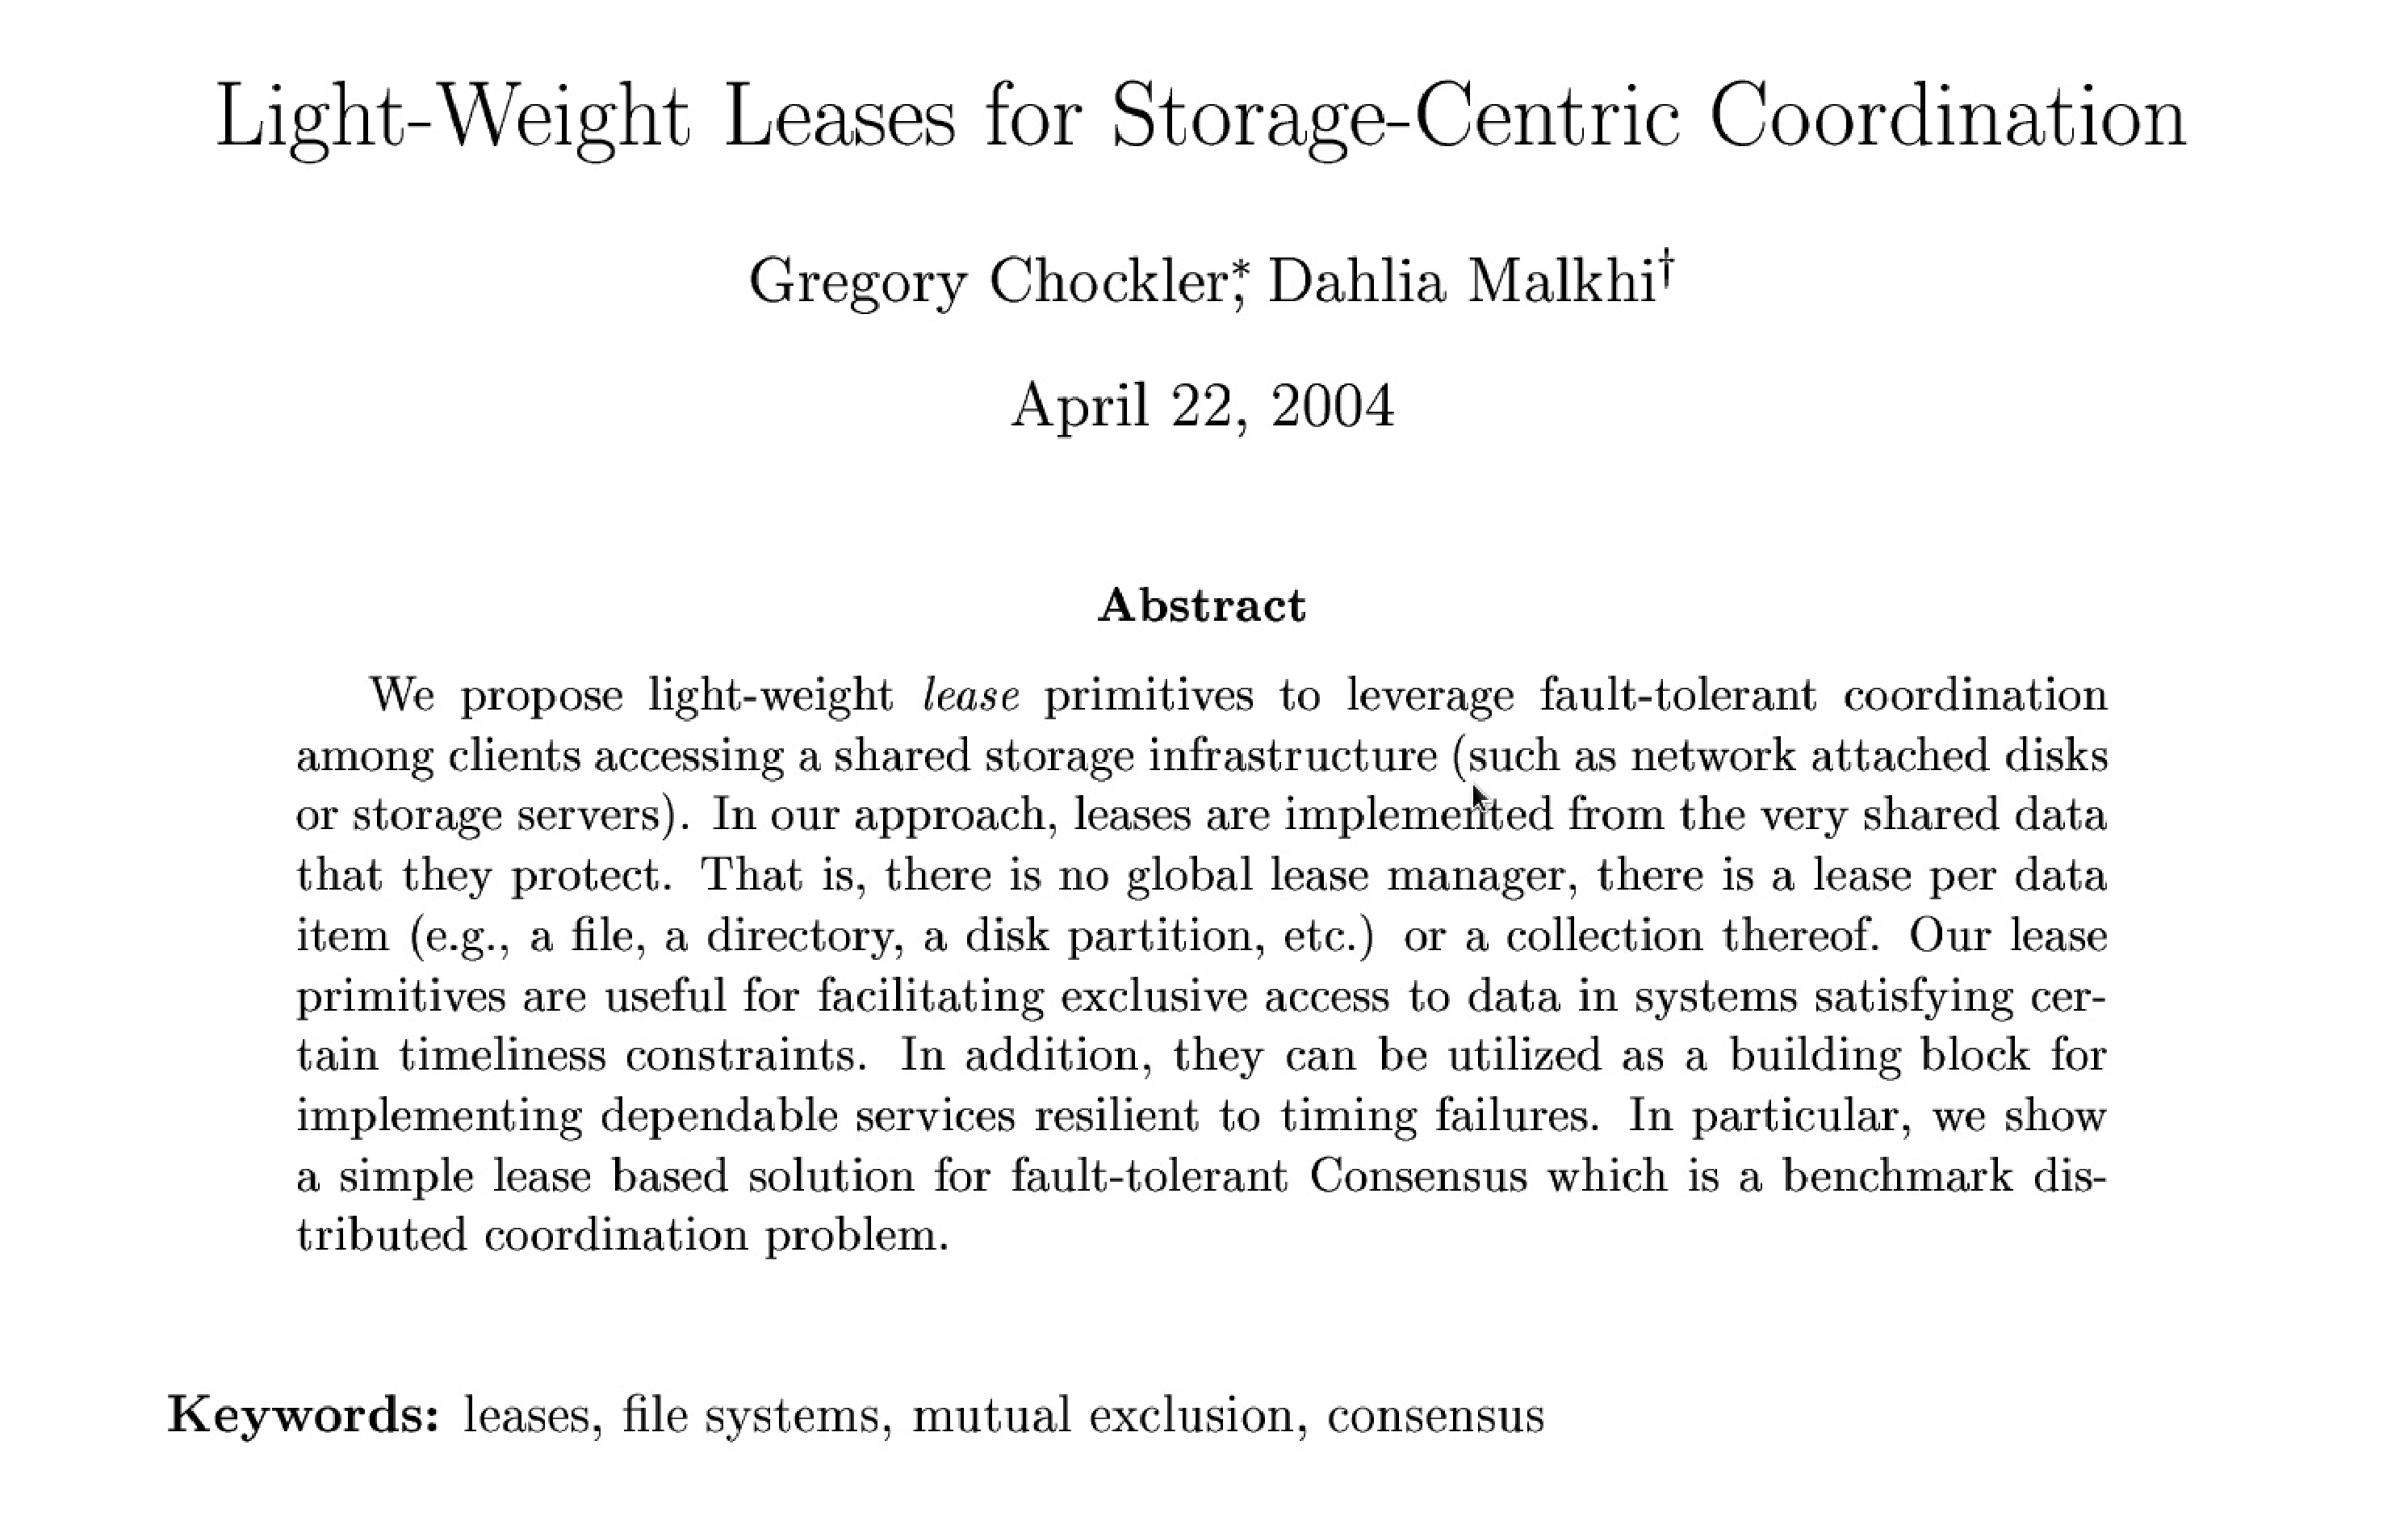
\includegraphics[height=5cm]{./img/delta-leases-paper.eps}
    \end{figure}
\end{frame}

\begin{frame}
    \frametitle{$\Delta$-Lease life cycle}
    \begin{figure}
        \centering
        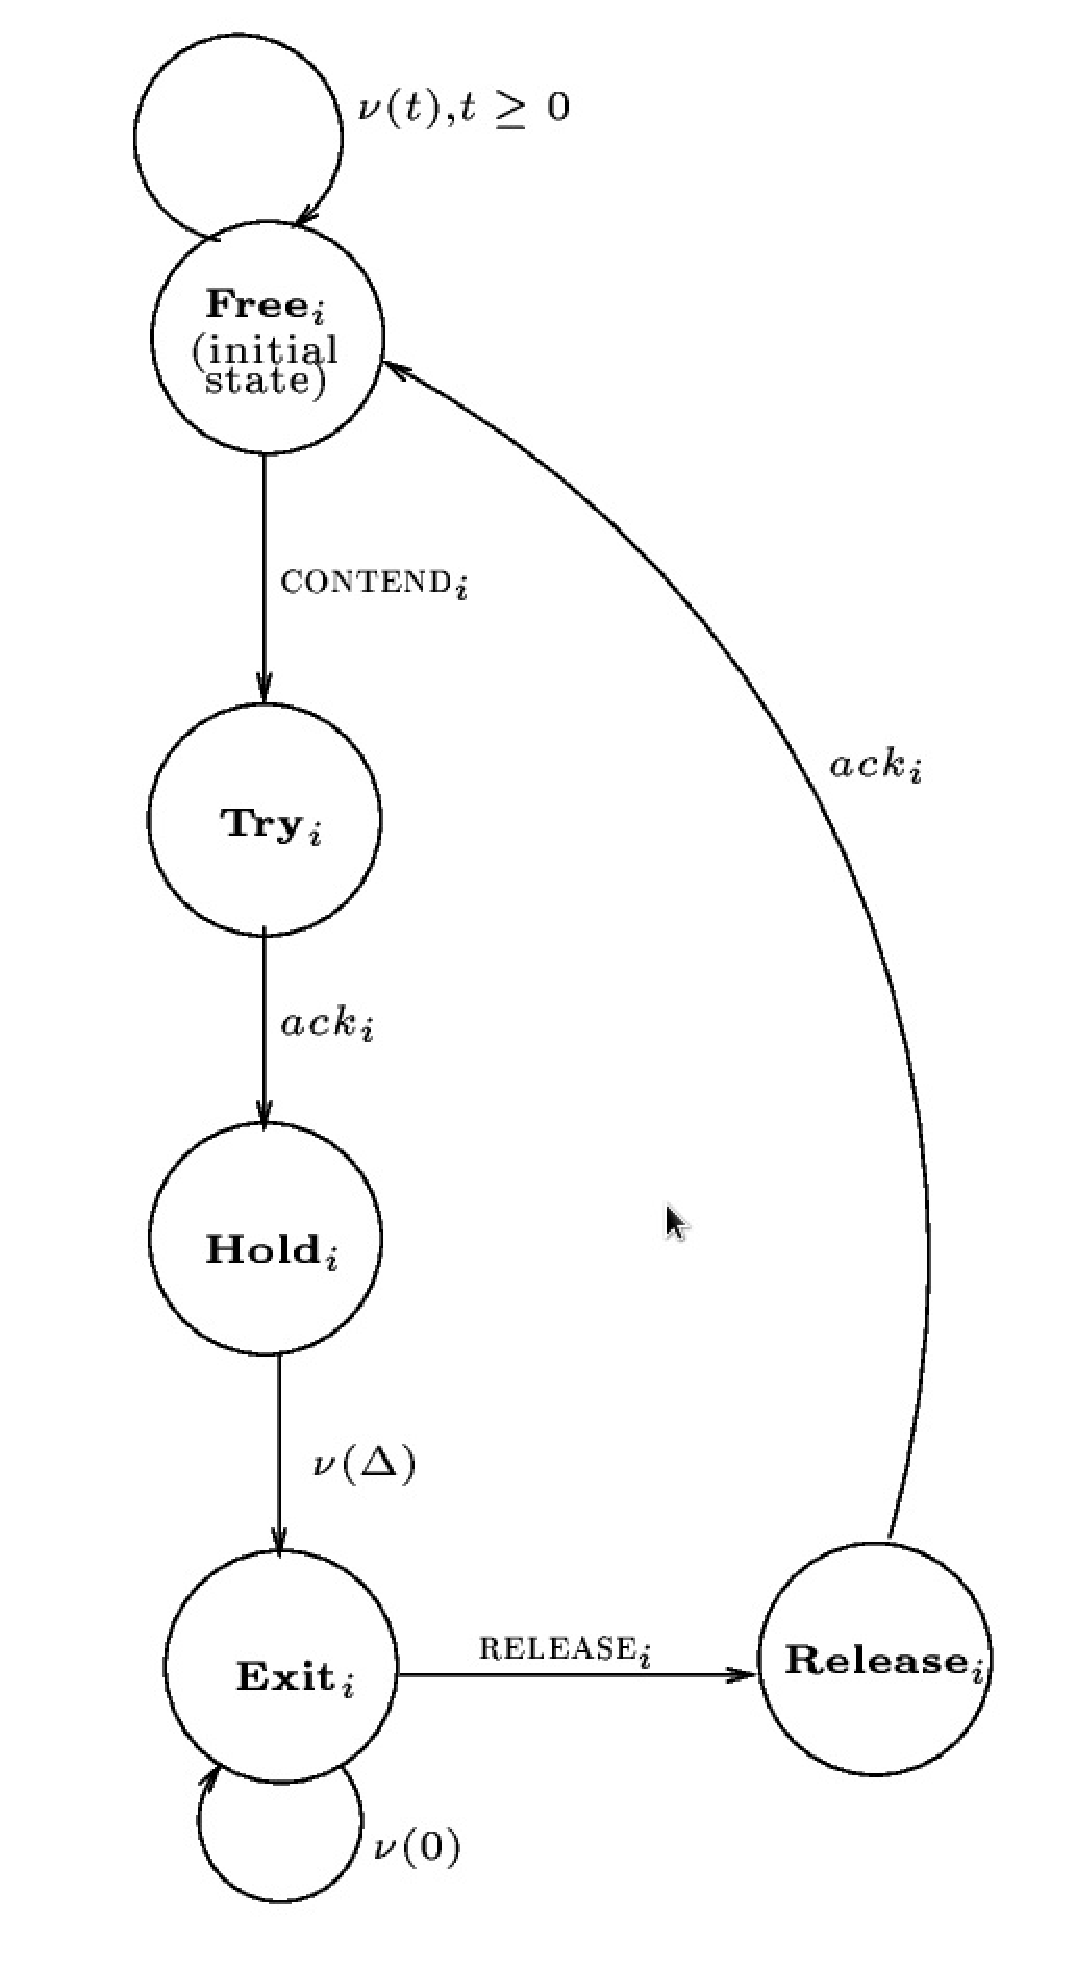
\includegraphics[height=5cm]{./img/delta-lease-life-cycle.eps}
    \end{figure}
    
    \centering
    \begin{itemize}
     \item Once acquired, lock is hold for time period $\Delta$.
     \item The time it takes for correct process to complete its access to do some operation on shared memory object (typically read/write) is strictly less than a known bound $\delta$ (known delay model).
    \end{itemize}
\end{frame}

\begin{frame}
    \frametitle{$\Delta$-Lease Implementation}
    \begin{figure}
        \centering
        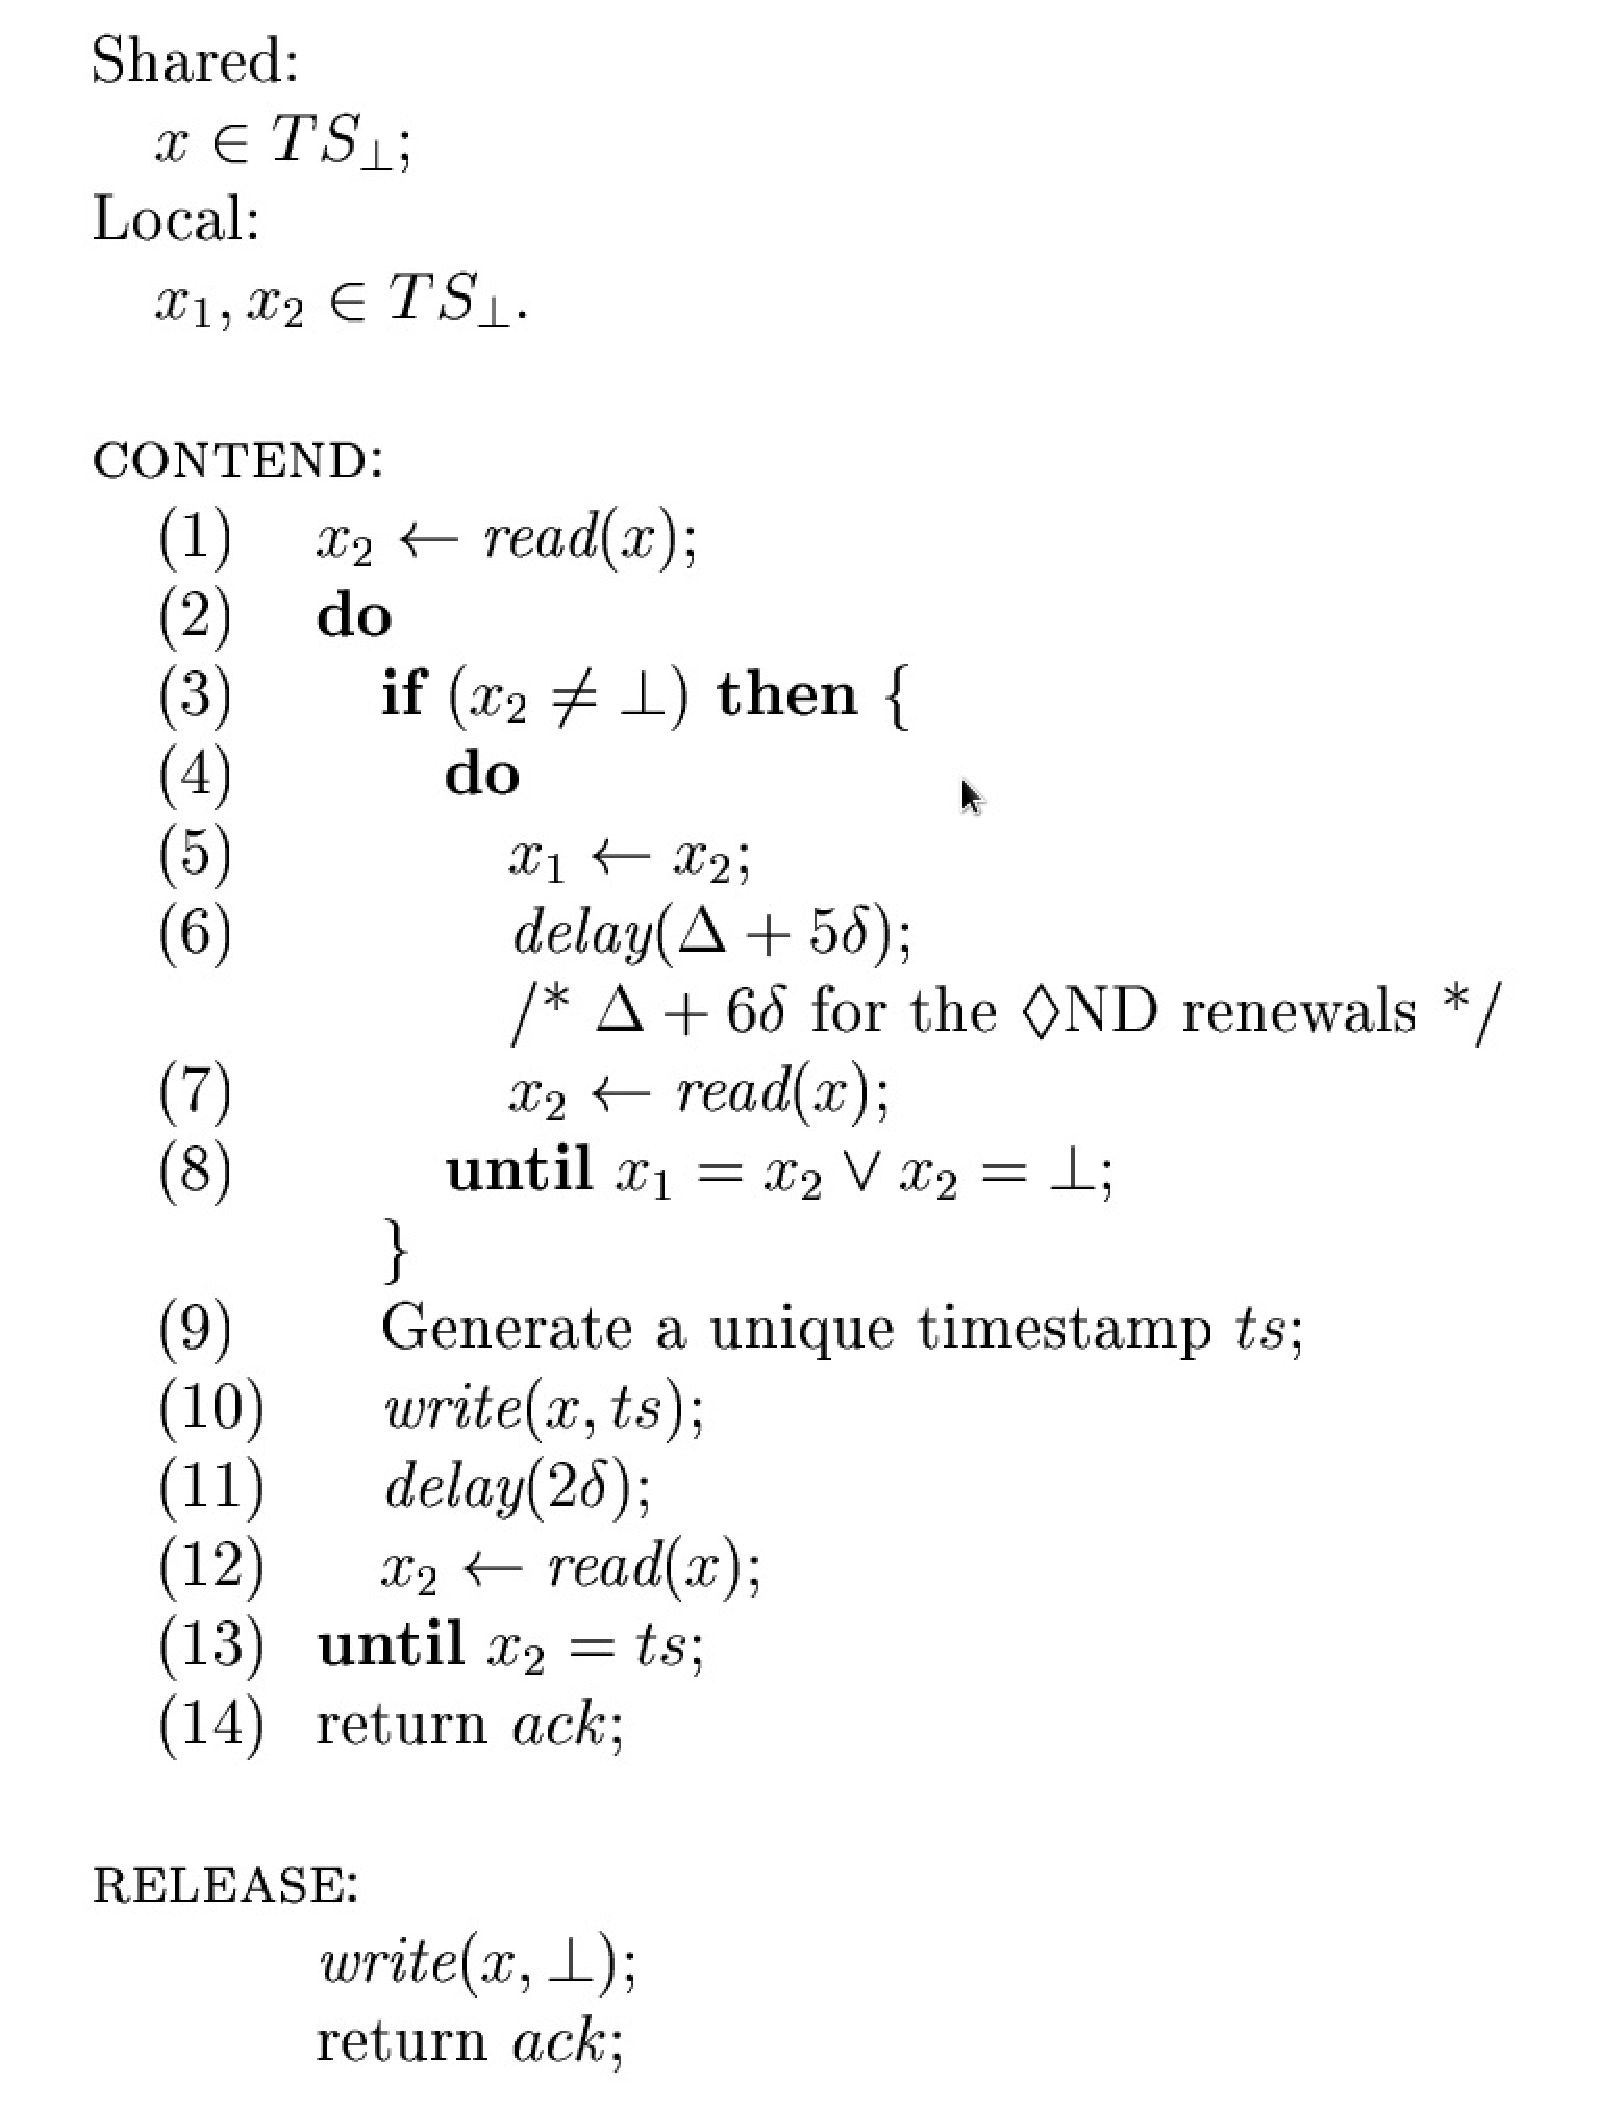
\includegraphics[height=7cm]{./img/delta-lease-alg.eps}
    \end{figure}
\end{frame}

\begin{frame}
    \frametitle{sanlock $\Delta$-Leases}
    \begin{itemize}
     \item $\Delta$-Leases are slow.
     \item For sanlock internal usage only.
     \item For keeping host ID
     \begin{itemize}
        \item Prevents two hosts to have same ID.
        \item Lease renewal is used also for checking is host is alive.
     \end{itemize}
    \end{itemize}
\end{frame}

\begin{frame}
    \frametitle{sanlock Disk Paxos leases}
    \begin{itemize}
     \item Fast to acquire.
     \item Provided to application to as general purpose application leases.
     \item Host IDs are used as Paxos leases owners.
    \end{itemize}
\end{frame}

\begin{frame}
    \frametitle{Summary}
    \begin{itemize}
     \item For locking the data on a shared storage lock located with data can be better solution than dedicated lock manager.
     \item There are various algorithms for storage-centric locks, e.g. Disk Paxos, a modification of classical Paxos algorithm.
     \item Disk Paxos itself is not sufficient for full implementation of shared disk locks and has to be used with some other algorithm, e.g. $\Delta$-Lease.
     \item Implementation of this approach can be found in sanlock project.
    \end{itemize}
\end{frame}

\begin{frame}
    \frametitle{Questions?}
    \centering
    \textbf{\Huge{Questions?}}
    
    \vspace{1cm}
    
    \centering
    \textbf{\dots read Disk Paxos and $\Delta$-Lease papers}:
    \vspace{0.5cm}
    \begin{itemize}
     \item \small\color{blue}\href{http://lamport.azurewebsites.net/pubs/disk-paxos-disc.pdf}{E. Gafni, L. Lamport, Disk Paxos}\color{black}
     \item \color{blue}\href{https://groups.csail.mit.edu/tds/papers/Chockler/TR934.ps}{G. Chockler, D. Malkhi, Light-Weight Leases for Storage-Centric Coordination}\color{black}
    \end{itemize}

\end{frame}
    
\end{document}
